\documentclass[11pt,class=report,crop=false]{standalone}
\usepackage[screen]{../python}

\begin{document}


%====================================================================
\chapitre{If ... then ...}
%====================================================================

\objectifs{The computer can react according to a situation. 
If a condition is met, it acts in a certain way, otherwise it does something else.}


%%%%%%%%%%%%%%%%%%%%%%%%%%%%%%%%%%%%%%%%%%%%%%%%%%%%%%%%%%%%%%%%
%%%%%%%%%%%%%%%%%%%%%%%%%%%%%%%%%%%%%%%%%%%%%%%%%%%%%%%%%%%%%%%%

\begin{cours}[If ... then ...]

Here's how to use the test \og{}\ci{if}\fg{} with \Python{}:
\index{if/then}
\index{if@\ci{if}}

\mybox{
\myfigure{0.7}{
  \tikzinput{fig-ifthen-lesson-1}
} }

Here is an example, which warns a driver if a variable \ci{speed} is too large.
\begin{center}
\begin{minipage}{0.7\textwidth}
\begin{lstlisting}
if speed > 110:
    print("Warning, you are driving too fast.")
\end{lstlisting}
\end{minipage} 
\end{center} 

Instructions can also be executed if the condition is not met using the keyword \og{}\ci{else}\fg{}.
\index{otherwise}
\index{else@\ci{else}}

\mybox{
\myfigure{0.7}{
  \tikzinput{fig-ifthen-lesson-2}
} }

Once again, it is the indentation that delimits the different blocks of instructions.
Here is an example that displays the sign of a number \ci{x}.
\begin{center}
\begin{minipage}{0.5\textwidth}
\begin{lstlisting}
if x >= 0:
    print("The number is positive (or zero).")
else:
    print("The number is negative.")
\end{lstlisting}
\end{minipage} 
\end{center} 


\end{cours}


%%%%%%%%%%%%%%%%%%%%%%%%%%%%%%%%%%%%%%%%%%%%%%%%%%%%%%%%%%%%%%%%
%%%%%%%%%%%%%%%%%%%%%%%%%%%%%%%%%%%%%%%%%%%%%%%%%%%%%%%%%%%%%%%%

\begin{cours}[Keyboard entry]

\index{enter@entry}

To be able to interact with the user, you can ask him to enter a text on the keyboard.
Here is a small program that asks for the user's first name and age and displays a message like \og{}Hello Kevin\fg{} then \og{}You are a minor/adult!\fg{} according to age.

\begin{center}
\begin{minipage}{0.6\textwidth}
\begin{lstlisting}
first_name = input ("What's your name? ")
print("Hello",first_name)

age_str = input("How old are you? ")
age = int(age_str)

if age >= 18:
    print("You're an adult!")
else:
    print("You're a minor!")
\end{lstlisting}
\end{minipage} 
\end{center} 

\emph{Explanations.}
\begin{itemize}
  \item The command \ci{input()}\index{input@\ci{input}}
  pauses the execution of the program and waits for the user to send a text (ended by pressing the \og{}Enter\fg{} key).
  
  \item This command returns a string.
  
  \item \index{int@\ci{int}} If you want an integer, you have to convert the string. For example, here \ci{age_str} can be equal to
  \ci{"17"} (it is not a number but a sequence of characters), while \ci{int(age_str)} is now the integer \ci{17}. 
  
  \item \index{str@\ci{str}} The reverse operation is also possible, \ci{str()} converts a number into a string. For example \ci{str(17)} returns the string \ci{"17"}; if you set \ci{age = 17}, then \ci{str(age)} also returns \ci{"17"}.
\end{itemize}

\end{cours}

%%%%%%%%%%%%%%%%%%%%%%%%%%%%%%%%%%%%%%%%%%%%%%%%%%%%%%%%%%%%%%%%
%%%%%%%%%%%%%%%%%%%%%%%%%%%%%%%%%%%%%%%%%%%%%%%%%%%%%%%%%%%%%%%%

\begin{cours}[The module \og{}random\fg{}]

% \index{random}
\index{random@\ci{random}}
\index{module!random@\ci{random}}

The \ci{random} module generates numbers as if they were randomly drawn.
\begin{itemize}
  \item Here is the command to place at the beginning of the program to call this module:
  \mycenterline{\ci{from random import *}}
  
  \item The command \ci{randint(a,b)}\index{randint@\ci{randint}} returns a random integer between $a$ and $b$.
  
  For example after the instruction \ci{n = randint(1,6)}, $n$ is a random integer with $1 \le n \le 6$.
  If you repeat the instruction \ci{n = randint(1,6)}, $n$ takes a new value. It's like rolling a 6-face dice.
  
  \item The command \ci{random()}, without argument, returns a floating number (i.e.~a decimal number) between $0$ and $1$.  
  For example, after the instruction \ci{x = random()}, then $x$ is a floating point number with $0 \le x < 1$.
\end{itemize}


\end{cours}


%%%%%%%%%%%%%%%%%%%%%%%%%%%%%%%%%%%%%%%%%%%%%%%%%%%%%%%%%%%%%%%%
% Activity 1
%%%%%%%%%%%%%%%%%%%%%%%%%%%%%%%%%%%%%%%%%%%%%%%%%%%%%%%%%%%%%%%%

\begin{activite}[Multiplication quiz]

\objectifs{Goal: program a small test on the multiplication tables.}

\begin{itemize}
  \item Define a variable $a$, to which you assign a random value between $1$ and $12$.
  
  \item Same thing for a variable $b$.
  
  
  \item Display the question on the screen: \og{}How much is the product  $a \times b$?\fg{}. (Replace $a$ and $b$ by their value!)
  
  \item Retrieve the user's answer and transform it into an integer.
  
  \item If the answer is correct, display \og{}Well done!\fg{}, otherwise display \og{}Lost! The correct answer was \ldots\fg{}.
\end{itemize}


\mybox{
\begin{minipage}{0.95\textwidth}
\textbf{Test of equality.} To test if two numbers $x$ and $y$ are equal, the instruction is:

\mycenterline{\ci{if x == y:}}

The equality test is written with the double symbol equal \og{}\ci{==}\fg{}.
For example \og{}\ci{x == 3}\fg{} returns \og{}True\fg{} if $x$ is equal to $3$ and \og{}False\fg{} otherwise.

Attention! The instruction \og{}\ci{x = 3}\fg{} has nothing to do with it, this instruction stores $3$ in the variable $x$.
\end{minipage}
}

\end{activite}


%%%%%%%%%%%%%%%%%%%%%%%%%%%%%%%%%%%%%%%%%%%%%%%%%%%%%%%%%%%%%%%%
% Activity 2
%%%%%%%%%%%%%%%%%%%%%%%%%%%%%%%%%%%%%%%%%%%%%%%%%%%%%%%%%%%%%%%%

\begin{activite}[The words of the turtle]

\objectifs{Goal: guide the turtle with a word, each character corresponding to an instruction.}

You give the \Python{} turtle a word, for example 
\mot{FlFrfflFrfF}, in which each character (read from left to right) corresponds to an instruction that the turtle must execute.

\begin{itemize}
  \item \mot{F} : go forward of $100$ by tracing,
  \item \mot{f} : go forward of $100$ without tracing,  
  \item \mot{l} : turn left by $90$ degrees,
  \item \mot{r} : turn right by $90$ degrees.
\end{itemize}

\emph{Example.}
Here is the drawing that the turtle must trace when
\mycenterline{\ci{word = "FflFlFrFlFFlfFF"}}

\begin{center}
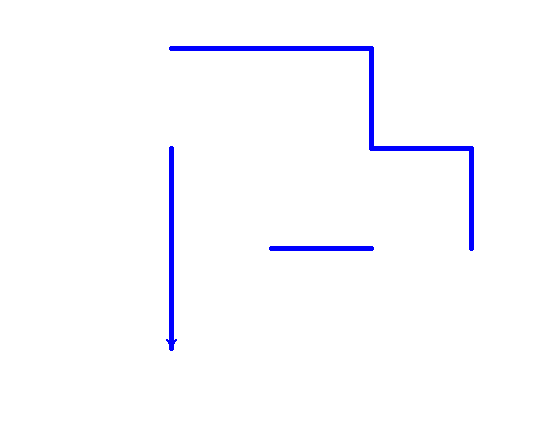
\includegraphics[scale=\myscale,scale=0.4]{screen-ifthen-2}
\end{center}

\emph{Hints.}
Here's how to scan the letters of a word and test if a letter is the character \mot{F}:
\begin{center}
\begin{minipage}{0.5\textwidth}
\begin{lstlisting}
for c in word:
    if c == "F":
        instructions...
\end{lstlisting}
\end{minipage} 
\end{center} 

   
\end{activite}



%%%%%%%%%%%%%%%%%%%%%%%%%%%%%%%%%%%%%%%%%%%%%%%%%%%%%%%%%%%%%%%%
%%%%%%%%%%%%%%%%%%%%%%%%%%%%%%%%%%%%%%%%%%%%%%%%%%%%%%%%%%%%%%%%

\begin{cours}[Booleans]
\sauteligne
\begin{itemize}
  \item A \defi{bolean}\index{boolean} is a data that is either equal to the value \og{}True\fg{} or the value \og{}False\fg{}. In \Python{} the values are \ci{True}\index{true@\ci{True}} and \ci{False}\index{false@\ci{False}} (with a capital letter).
  
  \item We obtain a boolean for example as a result of the comparison of two numbers.
  For example \ci{7 < 4} is equal to \ci{False} (because $7$ is not smaller than $4$). 
  Check that \ci{print(7 < 4)} displays \ci{False}.
  
  Here are the main comparisons:
  \begin{itemize}
    \item \textbf{Test of equality:}\quad \ci{a == b}\index{\ci{==}}
    	\item \textbf{Strict lower test:}\quad \ci{a < b}
    	\item \textbf{Large lower test:}\quad \ci{a <= b}\index{\ci{<=}}
    	\item \textbf{Higher test:}\quad \ci{a > b} \quad or \quad \ci{a >= b}\index{\ci{>=}}
    	\item \textbf{Test of non equality:}\quad \ci{a \!= b}\index{\ci{"!}\ci{=}}
  \end{itemize}
   
   For example \ci{6*7 == 42} is equal to \ci{True}.
   

   
   
   \item ~\index{assignment}\index{=@\ci{=}}
   \mybox{
   \begin{minipage}{0.95\textwidth}	
   \textbf{ATTENTION!}  
   The classic mistake is to confuse \og{}\ci{a = b}\fg{} and \og{}\ci{a == b}\fg{}.
   \begin{itemize}
     \item \textbf{Assignment.} \ci{a = b}
     puts the content of the variable \ci{b} in the variable \ci{a}.
     \item \textbf{Test of equality.} \ci{a == b} tests if the contents of \ci{a} and \ci{b} are the same, and is equal to \ci{True} or \ci{False}.
   \end{itemize}
	\end{minipage}
   }
   
  \item We can compare something other than numbers. For example,  
  \og{}\ci{char == "A"}\fg{} tests if the variable \ci{char} is equal to \ci{"A"}; \og{}\ci{its_raining == True}\fg{} tests if the variable \ci{its_raining} is true\ldots
  
  \item Booleans are useful in the test \og{}if \ldots{} then \ldots\fg{} and in the loops \og{}while \ldots{} then \ldots\fg{}.
  
  \item \textbf{Operations between booleans.}
  \index{logic operation}
  If $P$ and $Q$ are two booleans, new booleans can be defined.
  \begin{itemize}
    \item \textbf{Logical and.}\quad\og{}\ci{P and Q}\fg{}\index{and@\ci{and}} is true if and only if $P$ and $Q$ are true.
    	\item \textbf{Logical or.}\quad \og{}\ci{P or Q}\fg{}\index{or@\ci{or}} is true if and only if $P$ or $Q$ is true.
    	\item \textbf{Negation.}\quad \og{}\ci{not P}\fg{}\index{not@\ci{not}} is true if and only if $P$ is false.
  \end{itemize}  
  
  For example \og{}\ci{(2+2 == 2*2) and (5 < 3)}\fg{} returns \ci{False}, because
  even if we have $2+2 = 2 \times 2$, the other condition is not satisfied because $5 < 3$ is wrong.
  
  
  
\end{itemize}
\end{cours}




%%%%%%%%%%%%%%%%%%%%%%%%%%%%%%%%%%%%%%%%%%%%%%%%%%%%%%%%%%%%%%%%
% Activity 3
%%%%%%%%%%%%%%%%%%%%%%%%%%%%%%%%%%%%%%%%%%%%%%%%%%%%%%%%%%%%%%%%

\begin{activite}[Digits of an integer]

\objectifs{Goal: find numbers whose digits verify certain properties.}
\index{digits}

\begin{enumerate}
  \item The following program displays all integers from $0$ to $99$. Understand this program. What do the variables $u$ and $t$ represent?
  
\begin{center}
\begin{minipage}{0.5\textwidth}
\begin{lstlisting}
for t in range(10):
    for u in range(10):
        n  = 10*t + u
        print(n)
\end{lstlisting}
\end{minipage} 
\end{center} 
  
  \item Find all integers between $0$ and $999$ that check all the following properties:
  \begin{itemize}
    \item the integer ends with $3$,
    
    \item the sum of the digits is greater than or equal to $15$,
    
    \item the tens digit is even.
  \end{itemize}
   
  
  \item Modify your previous program to count and display the number of integers checking these properties.
  
\end{enumerate}

\end{activite}



%%%%%%%%%%%%%%%%%%%%%%%%%%%%%%%%%%%%%%%%%%%%%%%%%%%%%%%%%%%%%%%%
% Activity 4
%%%%%%%%%%%%%%%%%%%%%%%%%%%%%%%%%%%%%%%%%%%%%%%%%%%%%%%%%%%%%%%%

\begin{activite}[Triangles]

\objectifs{Goal: determine the properties of a triangle from the three lengths of the sides.}
\index{triangle}

We give ourselves three lengths $a$, $b$ and $c$. You will determine the properties of the triangle whose lengths would be $a$, $b$, $c$.

\myfigure{1.1}{
\tikzinput{fig-ifthen-1}
}  


Define three variables $a$, $b$ and $c$ with integer values and $a \le b \le c$ (or ask the user for three values).

\begin{enumerate}
  \item \textbf{Order.} Ask \Python{} to test if the lengths check $a \le b \le c$. Display a sentence for the answer.
  
  \item \textbf{Existence.} There is a triangle corresponding to these lengths if and only if:
  $$a + b \ge c.$$
  Ask \Python{} to test if this is the case and display the answer.
  
  
  \item \textbf{Rectangle triangle.} Ask \Python{} to test if the triangle is a rectangular triangle. (Think of Pythagoras' theorem.)
  
   \item \textbf{Equilateral triangle.} Test if the triangle is equilateral. 
   
   \item \textbf{Isosceles triangle.} Test if the triangle is isosceles.   
   
   \item \textbf{Acute triangle.} Tests if all angles are acute (i.e.~less than or equal to $90$ degrees).
   
    \emph{Hints.} 
    \begin{itemize}
      \item The cosine law allows to calculate an angle according to the lengths:
      
 \myfigure{1.1}{
\tikzinput{fig-ifthen-3}
}   
   
   $$\cos \alpha = \frac{-a^2+b^2+c^2}{2bc},
   \qquad
   \cos \beta = \frac{a^2-b^2+c^2}{2ac},
   \qquad
   \cos \gamma = \frac{a^2+b^2-c^2}{2ab}.$$   

   \smallskip
   
    \item To test if the angle $\alpha$ is acute just check $\cos \alpha \ge 0$ (in the end we never calculate $\alpha$, but only $\cos \alpha$).
   
   \end{itemize} 
   
\end{enumerate}   
     
    \smallskip 
     
    \objectifs{Find examples of lengths $a,b,c$ to illustrate the different properties.}
    
\end{activite}

\bigskip
\bigskip

%%%%%%%%%%%%%%%%%%%%%%%%%%%%%%%%%%%%%%%%%%%%%%%%%%%%%%%%%%%%%%%%
% Activity 5
%%%%%%%%%%%%%%%%%%%%%%%%%%%%%%%%%%%%%%%%%%%%%%%%%%%%%%%%%%%%%%%%

\begin{activite}[The mystery number]

\objectifs{Goal: code the essential game when learning to program. The computer chooses a random number. The user must guess this number by following the indications \og{}larger\fg{} or \og{}smaller\fg{} given by the computer. As this game is quickly boring, we introduce variants where the computer is allowed to lie or cheat!}


\begin{enumerate}
  \item \textbf{The classic game.}
  \begin{itemize}
    \item The computer randomly chooses a mystery number between $0$ and $99$.
    \item The player offers an answer.
    \item The computer replies 
    \og{}the number to find is greater\fg{} or
     \og{}the number to find is smaller\fg{} or
      \og{}bravo, it's the right number!\fg{}. 
     \item The player has seven attempts to find the right answer.
  \end{itemize}
  
  Program this game!
  
  \emph{Hints.} To leave a loop \ci{for} before the last proposal, you can use the command \ci{break}. Use this when the player finds the right answer.

  
  \item \textbf{The computer is lying.}
  
  To complicate the game, the computer has the right to lie from time to time.
  For example, about one in four times the computer gives the wrong indication \og{}larger\fg{}
  or \og{}smaller\fg{}.
  
  \emph{Hints.} To decide when the computer is lying, each turn, draw a random number between $1$ and $4$, if it is $4$ the computer will lie!
  
  
  
  
  \item \textbf{The computer is cheating.}
  
  Now the computer is cheating (but it no longer lies)! Each turn the computer changes a little bit the mystery number to find.
  
    \emph{Hints.} Each round, draw a random number, between $-3$ and $+3$ for example, and add it to the mystery number. (Be careful not to exceed the $0$ and $99$ limits.)
  
\end{enumerate}   
     
\end{activite}

\end{document}
